\section{Análisis distribucional}
\label{sec:analisis_distribucional}

% Distribuciones de cada variable con estadísticos descriptivos
% (media, mediana, IQR, outliers).
%
% Para cada variable: histograma o boxplot, media, mediana, desviación
% estándar, percentiles 5 y 95. Identificar variables con distribución
% degenerada (e.g. masa puntual, valores constantes por trial).
%
% Analizar por separado variables estáticas vs. dinámicas y, dentro
% de las dinámicas, la evolución a lo largo del trial (posición de
% fijación 1, 2, ..., k).
%
% Señalar variables candidatas a transformación (log, normalización)
% antes del modelado.

Se presenta el análisis distribucional de las variables.

El análisis se organiza en torno a dos perspectivas complementarias:
\begin{itemize}
    \item \textbf{Análisis global:} se presentan estadísticos descriptivos para cada variable, considerando el conjunto completo de fijaciones del dataset ($N = 61.252$). Esto permite identificar características generales de la distribución, como simetría, presencia de outliers o valores constantes.
    
    \item \textbf{Mirada por sujeto:} se examina la variabilidad de cada variable dentro de cada participante por separado. El Modelo de TRFs por regresión regularizada se estima de forma independiente para cada sujeto: la matriz de diseño de cada participante contiene únicamente sus propias fijaciones, y los coeficientes TRF resultantes reflejan la relación entre las variables y la señal cerebral de ese individuo. En consecuencia, es crucial verificar que las variables presentan variabilidad dentro de cada sujeto, ya que una variable constante para un participante no contribuirá a explicar su señal cerebral.
\end{itemize}


\subsection{Análisis global}
\subsubsection{Información Bottom Up}

Las variables de información bottom-up presentan asimetría positiva, con una mayoría de fijaciones que presentan valores bajos. Esto refleja que la mayoría de las fijaciones caen en zonas de baja saliencia.

\begin{table}[H]
\centering
\caption{Estadísticos descriptivos de las variables de información bottom-up.}
\label{tab:dist_bottomup}
\small
\setlength{\tabcolsep}{8pt}
\renewcommand{\arraystretch}{1.2}
\begin{tabular}{lrrr}
\toprule
 & \feat{saliencia\_media} & \feat{saliencia\_mediana} & \feat{saliencia\_pixel} \\
\midrule
count & 61252 & 61252 & 61252 \\
mean  & 0.1046 & 0.1004 & 0.0449 \\
std   & 0.1408 & 0.1391 & 0.0954 \\
min   & 0.0000 & 0.0000 & 0.0000 \\
25\%  & 0.0164 & 0.0157 & 0.0000 \\
50\%  & 0.0507 & 0.0471 & 0.0078 \\
75\%  & 0.1309 & 0.1255 & 0.0431 \\
max   & 0.9010 & 0.9059 & 1.0000 \\
\bottomrule
\end{tabular}
\end{table}

\subsubsection{Similitud con el target}

Al igual que las variables de información bottom-up, las variables de similitud con el target también presentan asimetría positiva, con una mayoría de fijaciones con valores bajos. Al igual que para las variables de saliencia, esto indica que la mayoría de las fijaciones caen sobre regiones de baja similitud con respecto a el target buscado.

\begin{table}[H]
\centering
\caption{Estadísticos descriptivos de las variables de similitud con el target.}
\label{tab:dist_similitud}
\small
\setlength{\tabcolsep}{8pt}
\renewcommand{\arraystretch}{1.2}
\begin{tabular}{lrrr}
\toprule
 & \feat{similitud\_media} & \feat{similitud\_mediana} & \feat{similitud\_pixel} \\
\midrule
count & 61252 & 61252 & 61252 \\
mean  & 0.0910 & 0.0835 & 0.0334 \\
std   & 0.1172 & 0.1157 & 0.0715 \\
min   & 0.0000 & 0.0000 & 0.0000 \\
25\%  & 0.0133 & 0.0118 & 0.0039 \\
50\%  & 0.0452 & 0.0373 & 0.0078 \\
75\%  & 0.1251 & 0.1098 & 0.0314 \\
max   & 0.8268 & 0.8353 & 0.9490 \\
\bottomrule
\end{tabular}
\end{table}

\subsubsection{Estado interno del proceso bayesiano}

Las variables del estado interno del proceso bayesiano presentan, en su mayoría,
distribuciones asimétricas positivas, concentradas en valores bajos y con colas largas hacia valores altos. El caso más extremo es \feat{posterior}, cuya probabilidad es marginal en la mayoría
de las fijaciones, seguido de \feat{ganancia\_informacion}, donde la mayoría de las
fijaciones aportan poca información sobre la localización del target. Las excepciones son \feat{evidencia\_visual} y
\feat{competencia\_fp\_media}, las únicas con distribuciones aproximadamente
simétricas. Las variables de entropía, por su parte, muestran que las escenas del
dataset tienen una complejidad visual relativamente homogénea
(\feat{entropia\_prior\_saliencia}) y que la posterior permanece casi uniforme
durante gran parte del trial (\feat{entropia\_posterior}), consistente con un proceso
de búsqueda que recién reduce su incertidumbre hacia las últimas fijaciones. Esta
dinámica temporal se analiza en detalle en la Sección~\ref{sec:coherencia_busqueda}.

\begin{table}[H]
\centering
\caption{Estadísticos descriptivos de las variables dinámicas del estado interno (parte I).}
\label{tab:dist_bayesiano_a}
\small
\setlength{\tabcolsep}{4pt}
\renewcommand{\arraystretch}{1.2}
\resizebox{\linewidth}{!}{%
\begin{tabular}{lrrrrr}
\toprule
 & \feat{evidencia\_visual} & \feat{competencia\_fp\_var} & \feat{competencia\_fp\_media} & \feat{competencia\_fp\_max} & \feat{posterior} \\
\midrule
count & 61252    & 61252   & 61252    & 61252         & 61252        \\
mean  & $-3.36$  & 4.60    & $-0.195$ & 4.83          & 0.0152       \\
std   & 2.28     & 1.58    & 0.0835   & 10.3          & 0.0939       \\
min   & $-8.91$  & 0.231   & $-0.342$ & ${\approx}0$  & ${\approx}0$ \\
25\%  & $-4.69$  & 3.50    & $-0.243$ & 0.0307        & 0.00000506   \\
50\%  & $-3.76$  & 4.50    & $-0.217$ & 0.484         & 0.0000230    \\
75\%  & $-2.71$  & 5.59    & $-0.183$ & 3.53          & 0.0000980    \\
max   & 8.44     & 13.6    & 0.298    & 74.2          & 1.00         \\
\bottomrule
\end{tabular}%
}
\end{table}


\begin{table}[H]
\centering
\caption{Estadísticos descriptivos de las variables del estado interno (parte II): entropías y ganancia.}
\label{tab:dist_bayesiano_b}
\small
\setlength{\tabcolsep}{8pt}
\renewcommand{\arraystretch}{1.2}
\begin{tabular}{lrrr}
\toprule
 & \feat{entropia\_prior\_saliencia} & \feat{entropia\_posterior} & \feat{ganancia\_informacion} \\
\midrule
count & 61252 & 61252   & 56751   \\
mean  & 5.45  & 5.35    & 0.214   \\
std   & 0.447 & 1.71    & 0.456   \\
min   & 3.85  & 0.0000140 & 0.00000300 \\
25\%  & 5.28  & 5.37    & 0.0257  \\
50\%  & 5.48  & 6.10    & 0.0517  \\
75\%  & 5.79  & 6.38    & 0.143   \\
max   & 6.15  & 6.58    & 5.90    \\
\bottomrule
\end{tabular}
\end{table}

\subsubsection{Calidad de la decisión}

Las tres variables de calidad de la decisión presentan asimetría positiva y revelan un patrón
consistente: si bien existen casos en los que el sujeto fija exactamente
la celda óptima, la mayoría de las fijaciones se alejan moderadamente del
óptimo, con una distancia mediana cercana a un tercio del ancho de la
imagen, y existen casos de suboptimalidad muy pronunciada. En conjunto,
estas variables evidencian una suboptimalidad sistemática: los sujetos no
siguen estrictamente la estrategia que utiliza el modelo nnELM. 

\begin{table}[H]
\centering
\caption{Estadísticos descriptivos de las variables de calidad de la decisión.}
\label{tab:dist_decision}
\small
\setlength{\tabcolsep}{8pt}
\renewcommand{\arraystretch}{1.2}
\begin{tabular}{lrrr}
\toprule
 & \feat{gap\_entropia} & \feat{distancia\_grilla} & \feat{distancia\_pixels} \\
\midrule
count & 56751  & 56751  & 56751  \\
mean  & 0.711  & 9.91   & 317    \\
std   & 1.04   & 6.03   & 193    \\
min   & 0.000  & 0.000  & 0.000  \\
25\%  & 0.127  & 5.39   & 172    \\
50\%  & 0.262  & 9.43   & 302    \\
75\%  & 0.702  & 13.9   & 446    \\
max   & 4.48   & 31.8   & 1016   \\
\bottomrule
\end{tabular}
\end{table}

\subsubsection{Competencia entre candidatos}

El análisis de las variables de competencia entre candidatos revela cómo si bien la mediana de \feat{competencia\_densidad} indica
que, en general, una única celda supera el umbral de dominancia (definido como el
$95\%$ del valor máximo del mapa EIG), el valor consistentemente alto de
\feat{competencia\_ratio} (media $=0.927$) muestra que el segundo mejor candidato
casi siempre se encuentra muy cerca del primero en magnitud. Es decir, aunque suele
haber un candidato que domina según el umbral elegido, el margen respecto al segundo
lugar es angosto. Esto podría ser indicio de que el umbral de $95\%$ resulta demasiado ácido:
un criterio más laxo posiblemente capturaría como candidatos a celdas que hoy quedan
justo por debajo del corte, incrementando la densidad de competencia reportada.
Ambas variables presentan además una cola larga hacia valores
extremos (\feat{competencia\_densidad} alcanza un máximo de $96$), lo que revela la
existencia de casos puntuales de fuerte ambigüedad, donde múltiples regiones compiten
de forma equivalente por la siguiente fijación.

\begin{table}[H]
\centering
\caption{Estadísticos descriptivos de las variables de competencia entre candidatos.}
\label{tab:dist_competencia}
\small
\setlength{\tabcolsep}{7pt}
\renewcommand{\arraystretch}{1.2}
\begin{tabular}{lrrr}
\toprule
 & \feat{competencia\_ratio} & \feat{competencia\_densidad} & \feat{competencia\_densidad\_norm} \\
\midrule
count & 61252  & 61252  & 61252   \\
mean  & 0.927  & 1.79   & 0.00233 \\
std   & 0.0562 & 1.82   & 0.00237 \\
min   & 0.763  & 1.00   & 0.00130 \\
25\%  & 0.889  & 1.00   & 0.00130 \\
50\%  & 0.940  & 1.00   & 0.00130 \\
75\%  & 0.974  & 2.00   & 0.00260 \\
max   & 1.00   & 96.0   & 0.125   \\
\bottomrule
\end{tabular}
\end{table}

\subsubsection{Análisis General}

La Figura~\ref{fig:violin_plot_features} presenta la distribución de las 
22 variables estandarizadas (z-score) mediante violinplots, agrupadas por 
categoría. La estandarización permite comparar la forma y dispersión 
relativa de todas las variables en un mismo eje, independientemente de 
sus unidades y escalas originales. Las líneas internas de cada violín 
indican la mediana y los cuartiles Q1 y Q3 de la distribución.

\begin{figure}[H]
    \centering
    \makebox[\textwidth][c]{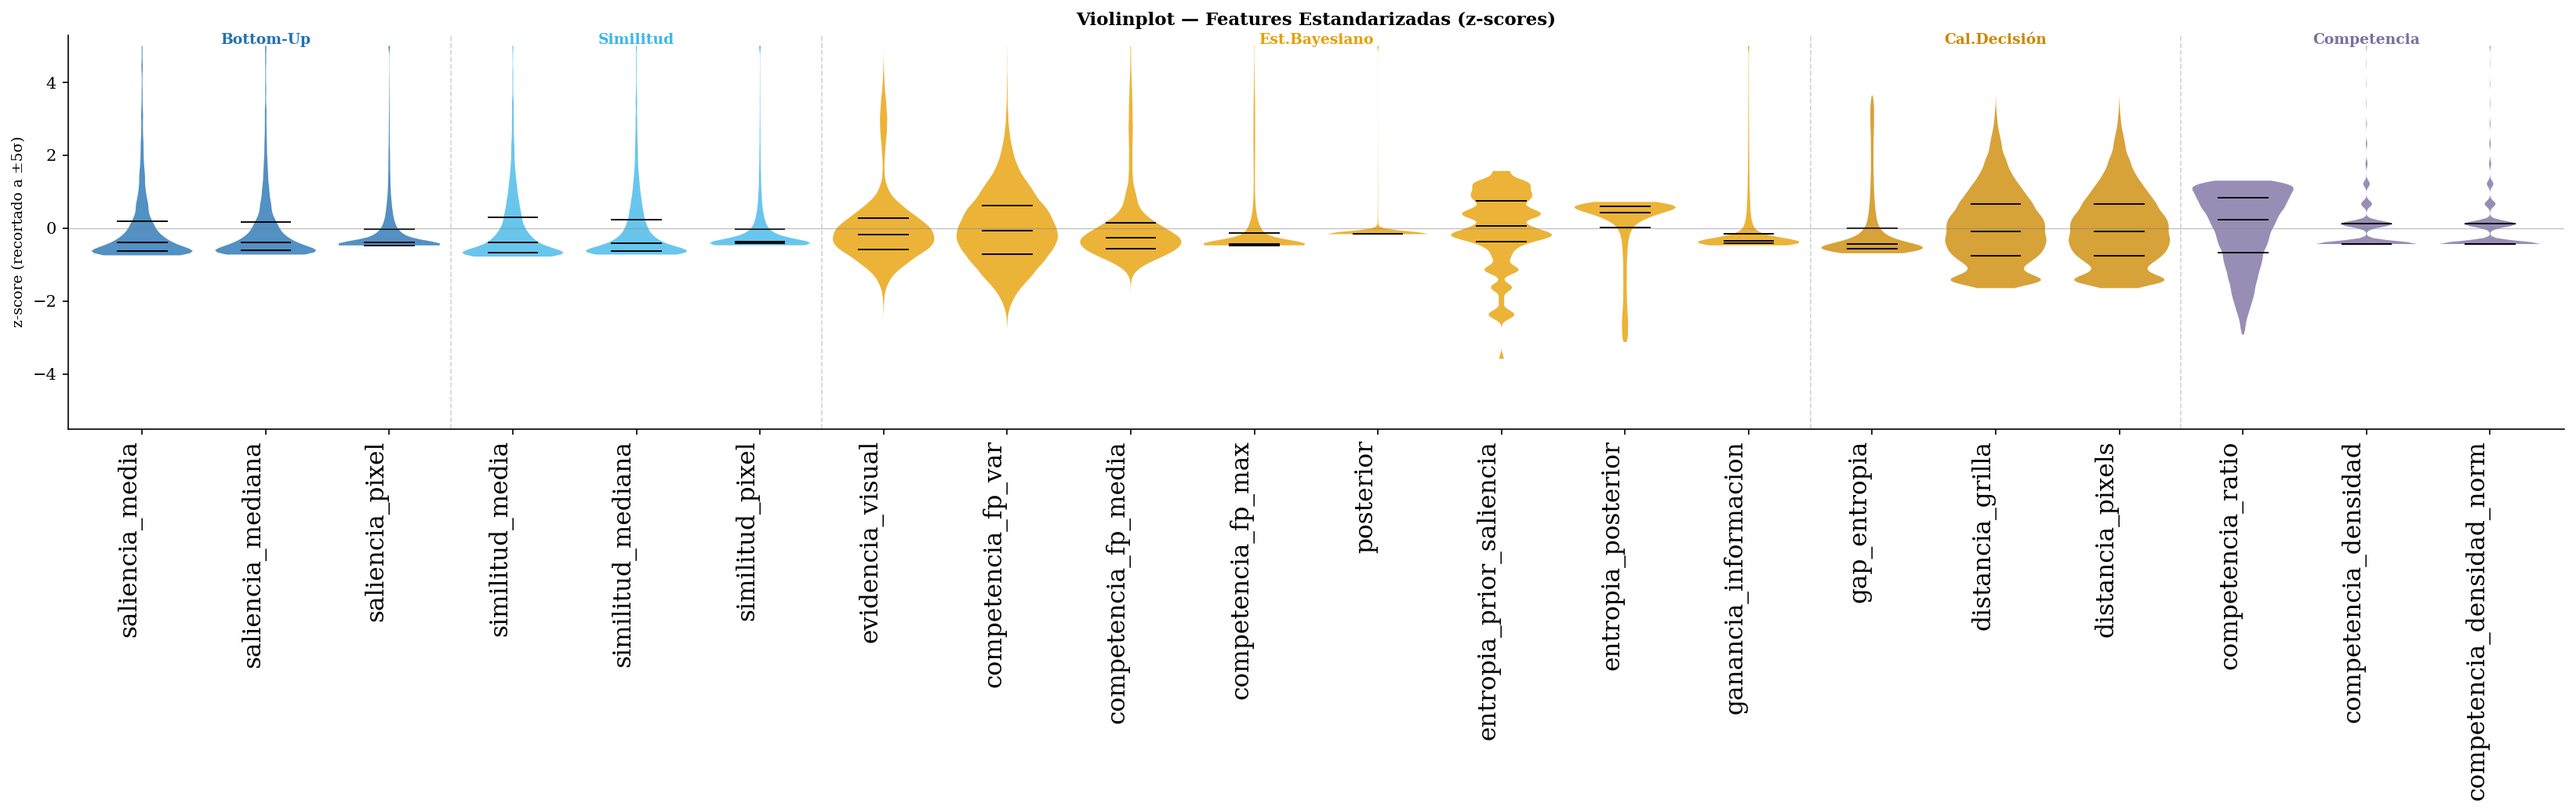
\includegraphics[width=1.3\textwidth]{chapters/04_extraccion_analisis_variables/images/violin_plot_features}}
    \caption{Distribución de las variables extraídas del modelo nnELM. Cada violín muestra la densidad empírica de la variable correspondiente sobre el conjunto completo de fijaciones ($N = 61.252$).}
    \label{fig:violin_plot_features}
\end{figure}


El análisis de los violinplots permite identificar patrones 
distribucionales relevantes que complementan los estadísticos 
descriptivos de las tablas anteriores. Se observan las diferencias en la forma de las 
distribuciones. Las variables que presentan distribuciones aproximadamente simétricas son \feat{evidencia\_visual}, \feat{competencia\_fp\_media}, \feat{competencia\_fp\_var}, \feat{distancia\_grilla} y \feat{distancia\_pixels}. El resto presenta asimetría en alguna 
dirección: las variables \feat{posterior}, \feat{ganancia\_informacion}, 
\feat{competencia\_fp\_max}, \feat{gap\_entropia} y 
\feat{competencia\_densidad} muestran una cola pronunciada hacia 
valores positivos, concentradas en valores bajos y eventos 
raros de valores altos. En sentido contrario, \feat{entropia\_posterior} 
y \feat{competencia\_ratio} presentan una cola hacia valores negativos, 
concentradas en valores altos dentro de su rango.

\subsection{Mirada por sujeto}

Lo relevante para el modelo de TRFs por regresión regularizada no es la dispersión
global del dataset sino la dispersión dentro de cada sujeto (variabilidad
\textit{within-subject}). El objetivo de esta sección es analizar cuánto varía cada variable dentro de las fijaciones de un mismo participante. Para cuantificarla se calcularon las siguientes métricas, tomando como unidad de análisis a cada sujeto por separado:

%\todo{Esto esta ok acá o debería ir en métodos?}

Para cada sujeto $s$ y cada variable $f$, se calculó el desvío estándar de los valores de $f$ sobre todas sus fijaciones:

\begin{equation}
    \sigma_{f,s} = \text{std}\left(\{f_t : t \in \text{fijaciones de } s\}\right).
\end{equation}

A partir de este valor se derivaron dos métricas de resumen:

\begin{itemize}
    \item \textbf{Std within-subject mediano} ($\widetilde{\sigma}_f$): 
    mediana de $\sigma_{f,s}$ entre los $S = 42$ sujetos. Cuantifica 
    cuánto varía típicamente la variable dentro de un participante, en 
    las unidades originales de la variable.

    \item \textbf{Coeficiente de variación within-subject mediano} 
    ($\widetilde{CV}_f$): mediana del cociente $\frac{\sigma_{f,s} }{\mu_{f,s}}$
    donde $\mu_{f,s}$ es la media de la variable para el sujeto $s$. Al 
    normalizar por la media, esta métrica es adimensional y permite 
    comparar variables en distintas escalas. Un valor de $\widetilde{CV}_f = 0.1$ 
    indica que el desvío estándar within-subject es el $10\%$ de la media.

\end{itemize}

La Tabla~\ref{tab:within_subject} presenta las tres métricas calculadas
para cada variable, ordenadas de menor a mayor coeficiente de variación
within-subject.

\begin{table}[H]
\centering
\caption{Variabilidad within-subject de cada variable}
\label{tab:within_subject}
\small
\setlength{\tabcolsep}{8pt}
\renewcommand{\arraystretch}{1.2}
\begin{tabular}{lrrl}
\toprule
\textbf{Variable} & $\widetilde{\sigma}_f$ & $\widetilde{CV}_f$ & \textbf{Categoría} \\
\midrule
\feat{competencia\_ratio}           & 0.0558  & 0.060 & Competencia       \\
\feat{entropia\_prior\_saliencia}   & 0.4461  & 0.082 & Est.\ Bayesiano   \\
\feat{entropia\_posterior}          & 1.6322  & 0.304 & Est.\ Bayesiano   \\
\feat{competencia\_fp\_var}         & 1.5731  & 0.342 & Est.\ Bayesiano   \\
\feat{competencia\_fp\_media}       & 0.0811  & 0.416 & Est.\ Bayesiano   \\
\feat{distancia\_pixels}            & 191.399 & 0.603 & Cal.\ Decisión    \\
\feat{distancia\_grilla}            & 5.9812  & 0.603 & Cal.\ Decisión    \\
\feat{evidencia\_visual}            & 2.2432  & 0.647 & Est.\ Bayesiano   \\
\feat{competencia\_densidad}        & 1.4914  & 0.822 & Competencia       \\
\feat{competencia\_densidad\_norm}  & 0.0019  & 0.822 & Competencia       \\
\feat{similitud\_media}             & 0.1150  & 1.278 & Similitud         \\
\feat{saliencia\_media}             & 0.1416  & 1.333 & Bottom-Up         \\
\feat{similitud\_mediana}           & 0.1137  & 1.369 & Similitud         \\
\feat{saliencia\_mediana}           & 0.1397  & 1.372 & Bottom-Up         \\
\feat{gap\_entropia}                & 1.0026  & 1.469 & Cal.\ Decisión    \\
\feat{ganancia\_informacion}        & 0.4512  & 2.111 & Est.\ Bayesiano   \\
\feat{saliencia\_pixel}             & 0.0959  & 2.123 & Bottom-Up         \\
\feat{competencia\_fp\_max}         & 9.9494  & 2.132 & Est.\ Bayesiano   \\
\feat{similitud\_pixel}             & 0.0718  & 2.133 & Similitud         \\
\feat{posterior}                    & 0.0874  & 6.468 & Est.\ Bayesiano   \\
\bottomrule
\end{tabular}
\end{table}

La variable \feat{competencia\_ratio} presenta el coeficiente de variación within-subject más bajo del conjunto ($\widetilde{CV} = 0.060$), consistente
con su distribución global estrecha ya observada en el análisis distribucional. Dado que esta variable es casi
constante tanto a nivel global como dentro de cada sujeto, se la considera
candidata a descarte antes del modelado de EEG. %\todo{Chequear si tiene sentido con los resultados en el modelo de TRFs. Ver si agregar esos resultados o ya la damos x descartada}

La variable \feat{entropia\_prior\_saliencia} también presenta un
$\widetilde{CV}$ bajo ($0.082$), pero es esperable al ser
estática por trial. Su variabilidad within-subject no refleja la dinámica 
de búsqueda fijación a fijación sino únicamente las diferencias entre las 
imágenes vistas por cada participante. La estrechez de su distribución global
frente al máximo teórico de $\ln(768) \approx 6.64$ refleja que las 
imágenes del dataset presentan una complejidad visual similar entre sí, 
lo que naturalmente limita la variabilidad de esta variable tanto entre 
trials como dentro de cada sujeto.

En el extremo opuesto, las variables de saliencia y similitud presentan 
coeficientes de variación superiores a $1$, lo que indica que su desvío 
estándar within-subject supera a su propia media. Lo mismo ocurre con 
\feat{ganancia\_informacion}, 
\feat{competencia\_fp\_max} y 
\feat{similitud\_pixel}. Estas variables 
presentan la mayor variabilidad relativa dentro de cada sujeto y son 
por lo tanto las candidatas más robustas como predictores individuales.

%Es importante considerar una limitación del coeficiente de variación como 
%métrica de variabilidad: al ser un cociente entre el desvío estándar y la 
%media, su valor se infla artificialmente cuando la media es cercana a cero 
%pero el desvío estándar no lo es proporcionalmente. En ese caso, un CV 
%alto no refleja necesariamente una variable con gran variabilidad 
%within-subject sino simplemente una variable cuya media es pequeña en 
%relación a su dispersión.
%
%Esta situación se presenta en \feat{posterior} ($\mu = 0.0135$, 
%$\widetilde{\sigma} = 0.087$), \feat{similitud\_pixel} ($\mu = 0.0337$, 
%$\widetilde{\sigma} = 0.072$) y \feat{saliencia\_pixel} ($\mu = 0.0450$, 
%$\widetilde{\sigma} = 0.096$): las tres tienen medias pequeñas pero 
%desvíos estándar considerablemente mayores que sus medias, lo que infla 
%el cociente. Esto contrasta con \feat{competencia\_densidad\_norm}, 
%que también tiene media pequeña ($\mu = 0.00231$) pero cuyos valores 
%están igualmente agrupados cerca de cero ($\widetilde{\sigma} = 0.0019$), 
%resultando en un CV moderado ($0.822$). Por esta razón, el CV de las 
%tres variables mencionadas debe interpretarse con cuidado y complementarse 
%con el análisis de su distribución global presentado en la sección 
%anterior.